

\section*{3. Mini - mundo, planteamiento a partir del modelo Entidad - Relación}

\subsection*{a. Números racionales}

\addcontentsline{toc}{subsection}{a. Números racionales}

\textbf{Diseña un modelo E/R para representar números racionales, bajo las siguientes consideraciones:}

\begin{itemize}
\item Cada número racional está determinado por dos números enteros: numerador y denominador.
\item Algunos de estos números son racionales reducidos de otros números racionales, por ejemplo, 1/4 es un racional reducido de 6/24. Se cumple que todo número racional tiene un único racional reducido (considera que solo se denomina racional reducido a aquel que ya está totalmente simplificado, es decir, 3/12 no sería un racional reducido).
\item Además de conocer el racional reducido asociado a cada fracción, se desea saber el factor de reducción asociado (en el caso anterior el factor de reducción sería 6).
\item Dos racionales se consideran diferentes si tienen el numerador o denominador distintos, aunque correspondan a la misma fracción reducida.
\end{itemize}
\subsubsection*{Análisis de requerimientos:}

Enumerar requerimientos candidatos (Entidades):
\begin{itemize}
\item Números Racionales
\end{itemize}

Comprensión del contexto del sistema (Relaciones):
\begin{itemize}
\item Todo número racional tiene un racional reducido (Cardinalidad 1:N).
\end{itemize}

Captura de requerimientos funcionales:
\begin{itemize}
\item Números Racionales
  \begin{itemize}
  \item Numerador.
  \item Denominador.
  \item Factor de reducción.
  \end{itemize}
\end{itemize}

Para la relación entre números racionales que asocia un racional con su número reducido, se consideró una relación parcial por parte de los números racionales reducidos, pues se menciona que no todos los números racionales son reducidos y una participación total por parte de los números racionales reducibles, pues se menciona que todos los números racionales tienen un racional reducido. A continuación se muestra el diagrama propuesto para esta situación.
\begin{figure}[H]
  \centering
  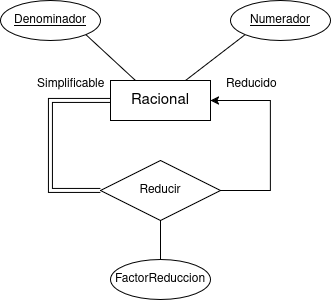
\includegraphics[width=0.5\textwidth]{imagenes/Racional.drawio.png}
\end{figure}
